\documentclass[department=cls, notes={hide notes}, official=true]{beamerruhuisstijl}

\title{Skipping meals, skipping words, and how the latter can benefit you and the first just makes you hungry}
\subtitle{Bayesian Language Modelling with Skipgrams}
\date{\today}
\author{lama-fan}

\usepackage{bbding}

\usepackage{cleveref}

\usepackage{tikz}
\usepackage{tkz-graph}
\usetikzlibrary[shapes,arrows,positioning,calc,patterns]

\usepackage{pgfplotstable}
\usepackage{pgfplots}
\pgfplotsset{compat=1.10}

\begin{document}

\begin{frame}
    \titlepage
\end{frame}
\note{

}

\begin{frame}{Bayesian Language Modelling with Skipgrams}
    \begin{block}{}
        Louis Onrust \\
        Centre for Language Studies, Radboud University \\
        Center for Processing Speech and Images, KU Leuven
    \end{block}

    \begin{block}{}
        \href{mailto:l.onrust@let.ru.nl}{l.onrust@let.ru.nl} \\
        \href{https://github.com/naiaden}{github.com/naiaden}
    \end{block}
\end{frame}
\note[itemize]{
}

\begin{frame}{Language Models}
	\begin{block}{Applications}
    	\begin{itemize}
        	\item Input assists on telephones
            \item Automatic translation of search results
            \item Digital court reporting
        \end{itemize}
    \end{block}
    
    \uncover<2->{
    \begin{block}{Flavours}
      \begin{itemize}
          \item Frequentist language models
          \item Bayesian language models
          \item Neural language models
          \item \ldots
      \end{itemize}
    \end{block}
    }
\end{frame}
\note{

}

\begin{frame}{The Task at Hand}
    \begin{center}
     	\emph{After all , tomorrow is another [\ldots]}
	\end{center}

    \begin{columns}[T] 
    	\uncover<2->{
        \begin{column}[T]{0.25\textwidth} 
            \begin{block}{Word prediction}
				\uncover<3->{
                \begin{itemize}
                	\item day
                \end{itemize}	
                }
            \end{block}
        \end{column}
   % }
   
        \begin{column}[T]{0.25\textwidth} 
       		\begin{block}{Word probability}
            	 \uncover<4->{
				\begin{itemize}
                	\item cow
                	\item day
                    \item vegetable
                    \item \ldots
                \end{itemize}
                }
            \end{block}
        \end{column}
        
        \begin{column}[T]{0.45\textwidth} 
       		\begin{block}{Pattern probability}
            	 \uncover<5->{
				\begin{itemize}
                	\item tomorrow is another day
                	\item tomorrow is another important
                    \item tomorrow is another race
                \end{itemize}
                }
            \end{block}
        \end{column}
    }
    \end{columns}
    
\pgfplotstableread[col sep=comma,header=true,row sep=crcr]{
word,freq\\
day,11\\
important,1\\
race,1\\
}\data
% \begin{center}
\medskip
\uncover<4->{
    \begin{tikzpicture}     
        \begin{axis}[    
            width=8cm,
            height=3.5cm,
            xbar,                                 
            xtick={0,5,10,15},    
            xmin=0,
            xmax=15,  
            nodes near coords, nodes near coords align={horizontal},
            symbolic y coords={day,important,race},
            xlabel={Observed frequency},
            y label style={at={(-0.1,0.5)}},
            enlarge x limits={abs=0},
            reverse legend,
        ]
        \addplot table [x=freq, y=word] {\data};
        \end{axis}
    \end{tikzpicture}
}
% \end{center}
\end{frame}

\begin{frame}{Generalising the $n$-gram}
	\begin{block}{$n$-grams}
    	\begin{itemize}
        	\item Continuous sequence of $n$ words
        \end{itemize}
    \end{block}
    
    \begin{block}{Skipgrams}
    	\begin{itemize}
        	\item $n$-gram with at most $n-2$ skips of length 1
        \end{itemize}
    \end{block}
    
    \begin{block}{Flexgrams}
    	\begin{itemize}
        	\item $n$-gram with any number of skips of any length
        \end{itemize}
    \end{block}
    \bigskip
    \begin{block}{Skipgrams in other works}
    	\begin{itemize}
        	\item[\PencilRightDown] A Generalized Language Model as the Combination of Skipped n-grams and Modified Kneser Ney Smoothing, Pickhardt et alia, 2014
            \item[\PencilRightDown] Skip-gram Language Modeling Using Sparse Non-negative Matrix Probability Estimation, Shazeer et alia, 2014
            \item[\XSolidBrush] Skipgrams in word2vec
        \end{itemize}
    \end{block}
\end{frame}

\begin{frame}{Backoff Patterns with Skipgrams}
	 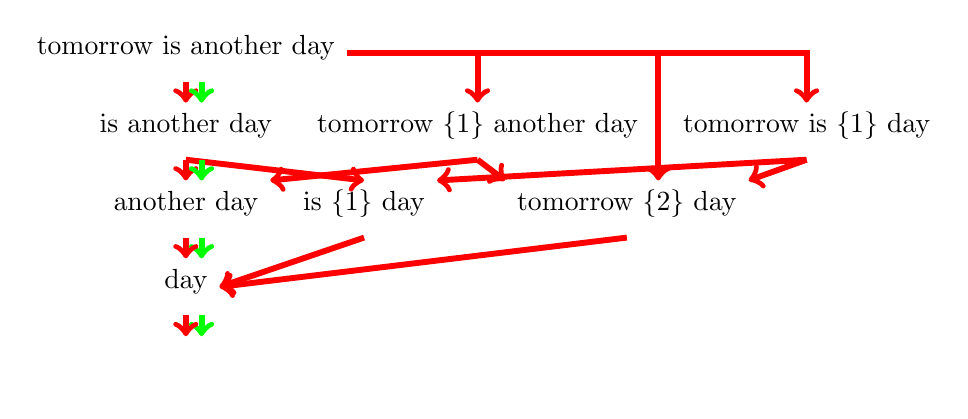
\begin{tikzpicture}[->,auto, node distance=0.75em,text centered,text height=1.5ex,text depth=1.25ex,line width=0.75mm]
	\node (abcd) {tomorrow is another day};
    
    
    \node[below = of abcd] (bcd) {is another day}; 
    \node[right = of bcd] (axcd) {tomorrow \{1\} another day};
	\node[right = of axcd] (abxd) {tomorrow is \{1\} day};
    \node[below = of bcd] (cd) {another day};
	
	\node[right = of cd] (bxd) {is \{1\} day};
    \node[below = of cd] (d) {day};
	\node[below = of d] (empty) {$\varnothing$};
    
    \node[xshift=0.6cm,right = of bxd] (axxd) {tomorrow \{2\} day};
    
    
    %%1
    
    \draw[red] let \p1 = (abcd.south), \p2 = (bcd.north) in (\x1,\y1) -- (\x2,\y2);
    \draw[red] let \p1 = (abcd.east), \p2 = (axcd.north) in (\x1,\y1) -| (\x2,\y2);
    \draw[red] let \p1 = (abcd.east), \p2 = (abxd.north) in (\x1,\y1) -| (\x2,\y2);
    \draw[red] let \p1 = (abcd.east), \p2 = ([xshift=0.4cm]axxd.north) in (\x1,\y1) -| (\x2,\y2);
    
    \draw[green] let \p1 = ([xshift=0.2cm]abcd.south), \p2 = ([xshift=0.2cm]bcd.north) in (\x1,\y1) -- (\x2,\y2);
    
%     \draw[blue] let \p1 = ([xshift=-0.2cm]abcd.south), \p2 = ([xshift=-0.2cm]bcd.north) in (\x1,\y1) -- (\x2,\y2);  
%     \draw[blue] let \p1 = ([yshift=0.2cm]abcd.east), \p2 = ([xshift=-0.2cm]axcd.north) in (\x1,\y1) -| (\x2,\y2);
%     \draw[blue] let \p1 = ([yshift=0.2cm]abcd.east), \p2 = ([xshift=-0.2cm]abxd.north) in (\x1,\y1) -| (\x2,\y2); 
%     \draw[blue] let \p1 = ([yshift=0.2cm]abcd.east), \p2 = ([xshift=0.2cm]axxd.north) in (\x1,\y1) -| (\x2,\y2);
    

	\draw[red] let \p1 = (axxd.south), \p2 = (d.east) in (\x1,\y1) -- (\x2,\y2);    
    
    
%     %%2
  
  \draw[red] let 	\p1 = (bcd.south), \p2 = (cd.north) in (\x1,\y1) -- (\x2,\y2);
    \draw[red] let 	\p1 = (bcd.south), 
    				\p2 = (bxd.north) in (\x1,\y1) -- (\x2,\y2);  
    \draw[red] let 	\p1 = (axcd.south), 
    				\p2 = (cd.north east) in (\x1,\y1) -- (\x2,\y2);    
    \draw[red] let 	\p1 = (abxd.south), 
    				\p2 = (bxd.north east)
                    	in (\x1,\y1) -- (\x2,\y2);
%     \draw[red] let 	\p1 = (bcd.south), \p2 = (cd.north) in (\x1,\y1) -- (\x2,\y2);
%     \draw[red] let 	\p1 = (bcd.south), 
%     				\p2 = (bxd.north), 
%                     \p3 = ([yshift=-0.35cm]bcd.south), 
%                     \p4 = ([yshift=0.15cm]bxd.north) 
%                     	in (\x1,\y1) -| (\x3,\y3) -| (\x4,\y4) -| (\x2,\y2);  
%     \draw[red] let 	\p1 = ([xshift=-0.1cm]axcd.south), 
%     				\p2 = ([xshift=0.4cm]cd.north), 
%                     \p3 = ([xshift=-0.1cm,yshift=-0.15cm]axcd.south), 
%                     \p4 = ([xshift=0.4cm,yshift=0.15cm]cd.north) 
%                     	in (\x1,\y1) -| (\x3,\y3) -| (\x4,\y4) -| (\x2,\y2);    
%     \draw[red] let 	\p1 = (abxd.south), 
%     				\p2 = (bxd.east)
%                     	in (\x1,\y1) |- (\x2,\y2);    
    
%     \draw[blue] let \p1 = ([xshift=-0.2cm]abxd.south), 
%     				\p2 = ([yshift=0.2cm]bxd.east)
%                     	in (\x1,\y1) |- (\x2,\y2);
%     \draw[blue] let \p1 = ([xshift=-0.2cm]bcd.south), 
%     				\p2 = ([xshift=-0.2cm]bxd.north), 
%                     \p3 = ([xshift=-0.2cm,yshift=-0.27cm]bcd.south), 
%                     \p4 = ([xshift=-0.2cm,yshift=0.27cm]bxd.north) 
%                     	in (\x1,\y1) -| (\x3,\y3) -| (\x4,\y4) -| (\x2,\y2);
                        
	\draw[red] let 	\p1 = (axcd.south), 
    				\p2 = (axxd.north west) in (\x1,\y1) -- (\x2,\y2);
                        
    \draw[red] let 	\p1 = (abxd.south), 
    				\p2 = (axxd.north east) in (\x1,\y1) -- (\x2,\y2);    
                        
%     \draw[blue] let \p1 = ([xshift=0.3cm]abxd.south), 
%     				\p2 = ([xshift=-0.2cm]axxd.north), 
%                     \p3 = ([xshift=0.3cm,yshift=-0.15cm]abxd.south), 
%                     \p4 = ([yshift=0.3cm,xshift=-0.2cm]axxd.north) 
%                     	in (\x1,\y1) -| (\x3,\y3) -| (\x4,\y4) -| (\x2,\y2);                     
    
    
	\draw[green] let \p1 = ([xshift=0.2cm]bcd.south), \p2 = ([xshift=0.2cm]cd.north) in (\x1,\y1) -- (\x2,\y2);
%     \draw[blue] let \p1 = ([xshift=-0.2cm]bcd.south), \p2 = ([xshift=-0.2cm]cd.north) in (\x1,\y1) -- (\x2,\y2);

%  %%3 
   
   
     \draw[green] let \p1 = ([xshift=0.2cm]cd.south), \p2 = ([xshift=0.2cm]d.north) in (\x1,\y1) -- (\x2,\y2); 
     \draw[red] let \p1 = (cd.south), \p2 = (d.north) in (\x1,\y1) -- (\x2,\y2); 
     \draw[red] let  \p1 = (bxd.south), 
     				 \p2 = (d.east)
     						in (\x1,\y1) -- (\x2,\y2);
%      \draw[blue] let \p1 = ([xshift=-0.2cm]bxd.south), 
%      				 \p2 = ([yshift=0.2cm]d.east)
%      						in (\x1,\y1) |- (\x2,\y2);
   
%    %%4
   
   
     \draw[green] let \p1 = ([xshift=0.2cm]d.south), \p2 = ([xshift=0.2cm]empty.north) in (\x1,\y1) -- (\x2,\y2);   
   \draw[red] let \p1 = (d.south), \p2 = (empty.north) in (\x1,\y1) -- (\x2,\y2);
   
   
   %%5
    
    
\end{tikzpicture}
\begin{block}{Backoff patterns}
    \begin{columns}[T] 
        \begin{column}[T]{0.3\textwidth} 
			\begin{itemize}
            	\item[simple] Only $n$-grams
            \end{itemize}
        \end{column}\hspace{-1.5cm}
        \begin{column}[T]{0.3\textwidth} 
			\begin{itemize}
            	\item[limited] All patterns until known pattern
            \end{itemize}
        \end{column}
        \begin{column}[T]{0.3\textwidth} 
			\begin{itemize}
            	\item[full] All patterns until words
            \end{itemize}
        \end{column}
    \end{columns}
\end{block}
\end{frame}

\begin{frame}{Probability Estimation}
	\begin{block}{Maximum Likelihood Estimate}
    	\[ p_{\text{ML}}(w_i | w_{i-N+1},\ldots,w_{i-1}) = \frac{C(w_{i-N+1},\ldots,w_{i})}{C(w_{i-N+1},\ldots,w_{i-1})} \]
        \begin{itemize}
        \item Parameter estimation is impossible for $N>2$
        \item Na\"ive priors assuming independent parameters fail as well
        \end{itemize}
    \end{block}
    
    \uncover<2->{
    \begin{block}{Smoothing}
    	\[ p_{\text{SM}}(w_i | w_{i-N+1},\ldots,w_{i-1}) = \sum_{n=1}^N\lambda(n)Q_n(w_i | w_{i-N+1},\ldots,w_{i-1}) \]
        \begin{itemize}
        	\item Chen and Goodman found that interpolated and modified
Kneser-Ney are best under virtually all circumstances
        \end{itemize}
    \end{block}
    }
\end{frame}

\begin{frame}{Bayesian Probability Estimation}
    \begin{block}{Parametrise conditional probabilities}
    \vspace*{-1em}
        \[ p(w_i = w | w_{i-N+1},\ldots,w_{i-1} = u) = G_u(w)\]
        \[ G_u = [G_u(w)]_{w\in W} \] 
        \[ \pi(w_{i-N+1},\ldots,w_{i-1}) = w_{i-N+2},\ldots,w_{i-1} \] \vspace*{-1em}
        \begin{itemize}
        	\item $G_u$ is a probability vector associated with context $u$
        \end{itemize}
    \end{block}
    
    \uncover<2->{
    \begin{block}{Hierarchical Dirichlet language model}
    	\begin{itemize}
        	\item What is $p(G_u|G_{\pi(u)})$?
            \item Standard Dirichlet distribution over probability vectors: does not outperform ikn and mkn (MacKay and Peto, 1994)
        \end{itemize}
    \end{block}
	}

	\uncover<3->{
	\begin{block}{Hierarchical Pitman-Yor process}
    	\begin{itemize}
        	\item Two-parameter extension of the Dirichlet distribution
            \item PYP produces power-law distributions
            \item Outperforms ikn and mkn (Teh, 2006)
        \end{itemize}
    \end{block}
    }
\end{frame}

\begin{frame}{Experimental Setup}
	
    \begin{columns}[T]
      \begin{column}[T]{0.4\textwidth}
        \begin{block}{Mixed-domain data}
          \begin{itemize}
            \item Google 1 Billion Words
            \item Wikipedia November 2013
          \end{itemize}
        \end{block}
      \end{column}\hspace{-0.5cm}
      \begin{column}[T]{0.65\textwidth}
        \begin{block}{Domain-specific data}
          \begin{itemize}
            \item JRC-ACQUIS: European legislation
            \item European Medicines Agency documents
          \end{itemize}
        \end{block}
      \end{column}

	\end{columns}
    \quad
   \begin{columns}[T]
      \begin{column}[T]{0.4\textwidth}
        \begin{block}{Sampling}
          \begin{itemize}
            \item[1bws] 10\% of the words
            \item[wps] 5\% of the words
          \end{itemize}
        \end{block}
      \end{column}\hspace{-0.5cm}
      \begin{column}[T]{0.65\textwidth}
        \begin{block}{Tresholding on 1BW}
          \begin{itemize}
            \item[unigrams] Threshold on 100: 99561 types
            \item[$n$-grams] Thresholds 2, 5, and 10
          \end{itemize}
        \end{block}
      \end{column}

	\end{columns}
    \quad
    \begin{block}{Method}
    \begin{itemize}
    	\item[cpyp] C++ library for nonparametric Bayesian modelling with Pitman-Yor process priors: \url{https://github.com/redpony/cpyp}
        \item[Colibri Core] C++ library for working with basic linguistic constructions such as n-grams and skipgrams: \url{https://github.com/proycon/colibri-core}
        \item[cococpyp] C++ toolkit for Bayesian language modelling: \url{https://github.com/naiaden/cococpyp}
    \end{itemize}
    \end{block}
\end{frame}

\pgfplotsset{every axis/.append style={
                    legend style={font=\tiny,line width=.75pt,mark size=2pt},
                    }}

\begin{frame}{Comparing the Models}
\begin{tikzpicture}
\begin{axis}[
	height=6cm, width=11cm, legend style={legend pos=south east},
  title=Relative change in perplexity w.r.t.\ HPYLM (test on Google 1BW),
  xmode = log,
  xmin=800,xmax=2048576000,
  ymin=-100,ymax=40,
  xlabel=Train corpus size (Google 1BW; in words),
  ylabel=$\Delta\%$]
\addplot table [x=N, y=Nngram]{bla.dat};
\addlegendentry{HPYLM}
\addplot table [x=N, y=Sngram]{bla.dat};
\addlegendentry{HPYLM+S simple}
\addplot table [x=N, y=Sbobaco]{bla.dat};
\addlegendentry{HPYLM+S limited}
\addplot table [x=N, y=Sglm]{bla.dat};
\addlegendentry{HPYLM+S full}
\addplot table [x=N, y=srilm]{bla.dat};
\addlegendentry{MKN};
\addplot +[mark=none] coordinates {(256000, -100) (256000, 40)};
%\addplot table [y=P, x=$Q_B$]{bla.dat};
%\addlegendentry{$Q_B$ series}
\end{axis}
\end{tikzpicture}

\end{frame}

\begin{frame}{Skipping Meals}
\begin{tikzpicture}
\begin{axis}[
	height=6cm, width=11cm, legend style={legend pos=north east},
  title=Effects of tresholding (test on Google 1BW),
  xmode = log,
  xmin=800,xmax=2048576000,
  %ymin=-100,ymax=40,
  xlabel=Train corpus size (Google 1BW; in words),
  ylabel=Perplexity]
\addplot table [x=N, y=W5Tt5]{bla1.dat};
\addlegendentry{W5Tt5 full}
\addplot table [x=N, y=W100Tt5]{bla1.dat};
\addlegendentry{W100Tt5 full}
\addplot table [x=N, y=W100Tt2]{bla1.dat};
\addlegendentry{W100Tt2 full}
\addplot table [x=N, y=W100Tt2bobaco]{bla1.dat};
\addlegendentry{W100Tt2 limited}
%\addplot table [y=P, x=$Q_B$]{bla.dat};
%\addlegendentry{$Q_B$ series}
\end{axis}
\end{tikzpicture}

\end{frame}

\begin{frame}{Learning Curves: Effects of Data Reduction}
\begin{tikzpicture}
\begin{axis}[
	height=6cm, width=11cm, legend style={legend pos=north east, fill=none},
  title=Testing on 1BW,
  xmode = log,
  xmin=800,xmax=2048576000,
  %ymin=-100,ymax=40,
  xlabel=Train corpus size (Google 1BW; in words),
  ylabel=Perplexity]
\addplot table [x=N, y=1bwnngram]{1bw.dat};
\addlegendentry{Tresholded HPYLM}
\addplot table [x=N, y=1bwsglm]{1bw.dat};
\addlegendentry{Tresholded HPYLM+S full}
\addplot table [x=N, y=1bwsnngram]{1bw.dat};
\addlegendentry{Sample HPYLM}
\addplot table [x=N, y=1bwssbobaco]{1bw.dat};
\addlegendentry{Sample HPYLM+S full}
%\addplot table [y=P, x=$Q_B$]{bla.dat};
%\addlegendentry{$Q_B$ series}
\end{axis}
\end{tikzpicture}

\end{frame}

\begin{frame}{Learning Curves: Effects of Data Reduction}
\begin{tikzpicture}
\begin{axis}[
	height=6cm, width=11cm, legend style={legend pos=north west, fill=none},
  title=Testing on JRC,
  xmode = log,
  xmin=800,xmax=2048576000,
  %ymin=-100,ymax=40,
  xlabel=Train corpus size (Google 1BW; in words),
  ylabel=Perplexity]
\addplot table [x=N, y=1bwnngram]{jrc.dat};
\addlegendentry{Tresholded HPYLM}
\addplot table [x=N, y=1bwsglm]{jrc.dat};
\addlegendentry{Tresholded HPYLM+S full}
\addplot table [x=N, y=1bwsnngram]{jrc.dat};
\addlegendentry{Sample HPYLM}
\addplot table [x=N, y=1bwssglm]{jrc.dat};
\addlegendentry{Sample HPYLM+S full}
%\addplot table [y=P, x=$Q_B$]{bla.dat};
%\addlegendentry{$Q_B$ series}
\end{axis}
\end{tikzpicture}

\end{frame}

\begin{frame}{Learning Curves: Effects of Data Reduction}
\begin{tikzpicture}
\begin{axis}[
	height=6cm, width=11cm, legend style={legend pos=north west, fill=none},
  title=Testing on EMEA,
  xmode = log,
  xmin=800,xmax=2048576000,
  %ymin=-100,ymax=40,
  xlabel=Train corpus size (Google 1BW; in words),
  ylabel=Perplexity]
\addplot table [x=N, y=1bwnngram]{emea.dat};
\addlegendentry{Treshold HPYLM}
\addplot table [x=N, y=1bwsglm]{emea.dat};
\addlegendentry{Treshold HPYLM+S full}
\addplot table [x=N, y=1bwsnngram]{emea.dat};
\addlegendentry{Sample HPYLM}
\addplot table [x=N, y=1bwssglm]{emea.dat};
\addlegendentry{Sample HPYLM+S full}
%\addplot table [y=P, x=$Q_B$]{bla.dat};
%\addlegendentry{$Q_B$ series}
\end{axis}
\end{tikzpicture}

\end{frame}

\begin{frame}{Learning Curves: Effects of Data Reduction}
\begin{tikzpicture}
\begin{axis}[
	height=6cm, width=11cm, legend style={legend pos=north west, fill=none},
  title=Testing on WP,
  xmode = log,
  xmin=800,xmax=2048576000,
  %ymin=-100,ymax=40,
  xlabel=Train corpus size (Google 1BW; in words),
  ylabel=Perplexity]
\addplot table [x=N, y=1bwnngram]{wp.dat};
\addlegendentry{Treshold HPYLM}
\addplot table [x=N, y=1bwsglm]{wp.dat};
\addlegendentry{Treshold HPYLM+S full}
\addplot table [x=N, y=1bwsnngram]{wp.dat};
\addlegendentry{Sample HPYLM}
\addplot table [x=N, y=1bwssbobaco]{wp.dat};
\addlegendentry{Sample HPYLM+S limited}
%\addplot table [y=P, x=$Q_B$]{bla.dat};
%\addlegendentry{$Q_B$ series}
\end{axis}
\end{tikzpicture}

\end{frame}
%			

\begin{frame}{Contribution of Skipgrams}

\begin{columns}[b]
		\begin{column}[b]{0.1\textwidth}
            	\begin{block}{\strut}
                \begin{tabular}{l}
                      \\
					jrc \\
                    1bw\\
                    1bws\\
                    emea\\
                    wps \\
                    \end{tabular}
                \end{block}
                \vspace{0pt}
    		\end{column}
			\begin{column}[b]{0.4\textwidth}
            	\begin{block}{HPYLM}
                \begin{tabular}{llllllll}
                     jrc  & 1bw   & emea & wp   \\
					 13 & 1195 & 961 & 1011 \\
                     1232 & 171 & 1749 & 724 \\
                     768 & 158 & 946 & 493 \\
                     600 & 1143 & 4 & 843 \\ 
                    555 & 455 & 1005 & 217 \\
                    \end{tabular}
                \end{block}
                \vspace{0pt}
    		\end{column}
            \quad
        	\begin{column}[b]{0.4\textwidth}
            	\begin{block}{HPYLM + Skipgrams}
				\begin{tabular}{llllllll}
                         jrc  & 1bw   & emea & wp   \\
                     13 & 1162 & 938 & 1008 \\
                      \textbf{\textit{728}} & \textbf{\textit{81}} & \textbf{\textit{1069}} & \textbf{\textit{542}} \\
                     751 & 162 & 921 & 507 \\
                     581 & 1155 & 4 & 842 \\
                     565 & 470 & 990 & 227 \\
                \end{tabular}
                \end{block}
                \vspace{0pt}
    		\end{column}       
        \end{columns}
 
\end{frame}

\begin{frame}{Preliminary conclusions}

\begin{block}{Sampled versus tresholded corpus}
\begin{itemize}
\item For in-domain evaluation we need about 2 times the amount of tresholded data
\item For cross-domain evaluation we need at least 5 times as much data
\end{itemize}
\end{block}

\begin{block}{When to use tresholding}
\begin{itemize}
\item Within-domain better with tresholding, because more training data (patterns) like test data
\item Cross-domain better without tresholding, because more types (100k vs.\ 1.1M types)
\end{itemize}
\end{block}

\begin{block}{Skipgrams help in all situations}
\begin{itemize}
\item Within-domain performance converges with ngrams
\item Cross-domain performance increases (30-40\% reduction in perplexity)
\end{itemize}
\end{block}

\begin{block}{Intrinsic evaluation}
	\begin{itemize}
    	\item Apply HPYLM+S to ASR, MT, \ldots
    \end{itemize}
\end{block}

\end{frame}





\begin{frame}{Choosing a Language Model}
	\begin{block}{Quick turnaround}
    	\begin{itemize}
    	\item[\PencilRightDown] Improved backing-off for m-gram language modeling, Kneser \& Ney, 1995
        \end{itemize}
    \end{block}
    
    \begin{block}{Best results}
    	\begin{itemize}
    	\item[\PencilRightDown] Hierarchical Pitman-Yor process language model, Teh, 2006
        \item[\PencilRightDown] A parallel training algorithm for hierarchical Pitman-Yor process language models, Huang \& Renals, 2009
		\item[\PencilRightDown] Recurrent neural network language model, Mikolov et alia, 2010
		\end{itemize}
\end{block}
    
    \begin{block}{Newest}
    	\begin{itemize}
          \item[\PencilRightDown] Sparse Non-negative Matrix Language Modeling For Skip-grams, Shazeer et alia, 2014
          \item[\PencilRightDown] Language Modeling with Power Low Rank Ensembles, Parikh et alia, 2014
          \item[\PencilRightDown] Word representations via Gaussian embedding, Vilnis and MacCallum, under review
       \end{itemize}
    \end{block}

\end{frame}

\end{document}

%http://stats.stackexchange.com/questions/22/bayesian-and-frequentist-reasoning-in-plain-english